\documentclass[12pt,a4paper]{article} 

\usepackage{fn2kursstyle}
\usepackage[russian]{babel}
\usepackage[T2A]{fontenc} 
\usepackage[utf8]{inputenc} 
\usepackage{geometry}
\usepackage{graphicx}
\usepackage{mathtools}
\usepackage{tikz}
\usepackage{pdfpages}
\usepackage{booktabs}
\usepackage{multirow,array}
\usepackage{siunitx}
\usepackage{amsmath}
\usepackage[hidelinks]{hyperref}

\counterwithout{equation}{section}
\counterwithout{figure}{section}
\graphicspath{{pic/}}
\frenchspacing 

\newcolumntype{C}[1]{>{\centering\arraybackslash}p{#1}}

\newcommand{\picref}[1]{рис. \ref{#1}}
\newcommand{\tabref}[1]{таблица \ref{#1}}
\newcommand{\half}{\frac{1}{2}}
\newcommand{\dhalf}{\dfrac{1}{2}}
\newcommand*{\Scale}[2][4]{\scalebox{#1}{$#2$}}

\title{Лабораторная работа №1 по дисциплине "Разработка программных комплексов" на тему "Проекционные методы"}
\group{ФН2-72Б}
\author{Токарев А.\,И.}
\supervisor{Азметов Х.\,Х.}
\date{2022}

\begin{document}
    \maketitle
    \tableofcontents
    \pagebreak

    \section{Задача}

    Создать программу решения дифференциального уравнения проекционными методами. Задано урванение на области $[0, 1]\colon$
    \[
        \dfrac{d^2 u}{dx^2} + u + x = 0, \quad u(0) = u(1) = 0.
    \]  

    Необходимо реализовать методы решения:
    \begin{enumerate}
        \item Метод коллокаций в точках
        \item Метод коллокаций в подобластях
        \item Метод Бубнова-Галеркина
        \item Метод Галеркина
        \item Метод наименьших квадратов
        \item Метод Ритца
    \end{enumerate}

    Для каждого из методов нужно получить решение с порядком аппроксимации от $1$ до $3$.

    \pagebreak

    \section{Метод коллокации в точке}

    \begin{center}
        \begin{tabular}{|c|c|c|} 
         \hline
         № & Норма ошибки & Коэффициенты \\ 
         \hline
         1 & $0.12$ & $a_1=0.286$ \\ 
         \hline
         2 & $0.0117$ & $a_1=0.195, a_2=0.17$ \\ 
         \hline
         3 & $8\cdot10^{-4}$ & $a_1=0.19, a_2=0.196, a_3=-0.02$ \\ 
         \hline
         4 & $5\cdot10^{-5}$ & $a_1=0.1883, a_2=0.1887, a_3=-0.105, a_4 =-0.008$ \\ 
         \hline
         5 & $3\cdot10^{-6}$ & $a_1=0.1884, a_2=0.1883, a_3=-0.0094, a_4=-0.0102, a_5=0.0008$ \\ 
         \hline
        \end{tabular}
    \end{center}

    \begin{figure}[h]
        \centering
        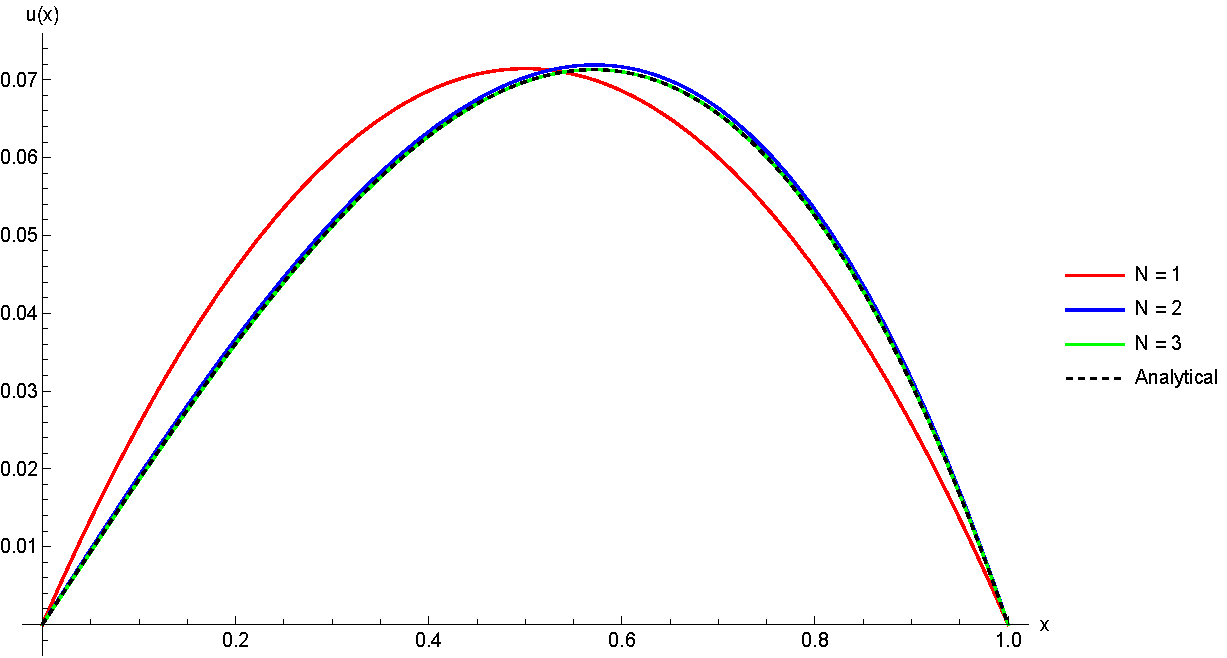
\includegraphics[width=0.7\textwidth]{1.pdf}
        \caption{График полученных решений при различных N}
    \end{figure}
    \begin{figure}[h]
        \centering
        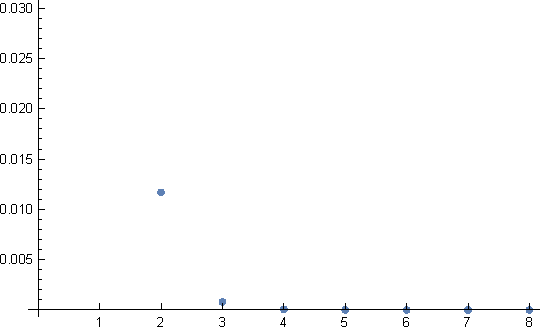
\includegraphics[width=0.5\textwidth]{1_error.pdf}
        \caption{График ошибок}
    \end{figure}

    \pagebreak

    \section{Метод коллокаций в подобластях}

    \begin{center}
        \begin{tabular}{|c|c|c|} 
         \hline
         № & Норма ошибки & Коэффициенты \\ 
         \hline
         1 & $0.117$ & $a_1=0.27$ \\ 
         \hline
         2 & $0.02$ & $a_1=0.1876, a_2=0.17$ \\ 
         \hline
         3 & $8\cdot10^{-4}$ & $a_1=0.1882, a_2=0.193, a_3=-0.023$ \\ 
         \hline
         4 & $4\cdot10^{-5}$ & $a_1=0.1884, a_2=0.1886, a_3=-0.01, a_4=-0.0086$ \\ 
         \hline
         5 & $1.5\cdot10^{-6}$ & $a_1=0.1883, a_2=0.1883, a_3=-0.0094, a_4=-0.0102, a_5=0.0008$ \\ 
         \hline
        \end{tabular}
    \end{center}

    \begin{figure}[h]
        \centering
        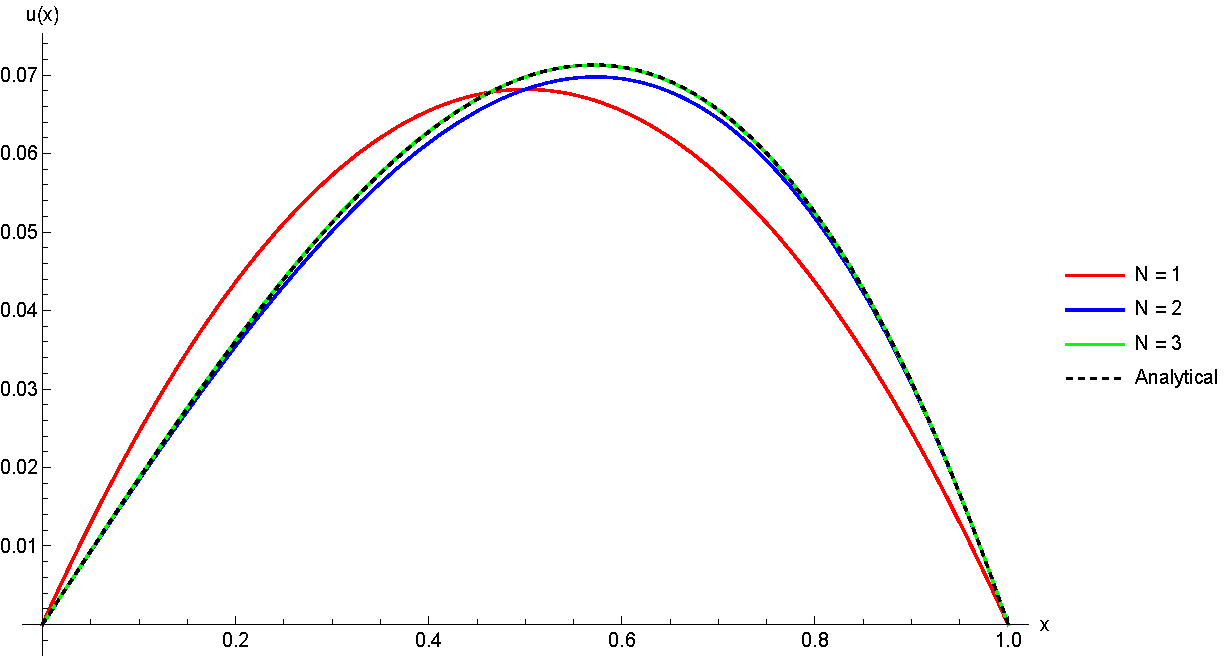
\includegraphics[width=0.7\textwidth]{2.pdf}
        \caption{График полученных решений при различных N}
    \end{figure}
    \begin{figure}[h]
        \centering
        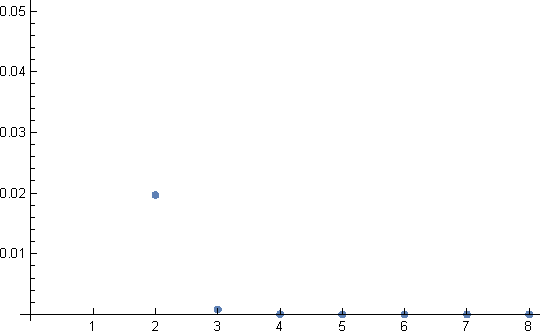
\includegraphics[width=0.5\textwidth]{2_error.pdf}
        \caption{График ошибок}
    \end{figure}

    \pagebreak

    \section{ Метод Бубнова-Галеркина}

    \begin{center}
        \begin{tabular}{|c|c|c|} 
         \hline
         № & Норма ошибки & Коэффициенты \\ 
         \hline
         1 & $0.115$ & $a_1=0.2778$ \\ 
         \hline
         2 & $0.004$ & $a_1=0.1924, a_2=0.1707$ \\ 
         \hline
         3 & $3\cdot10^{-4}$ & $a_1=0.1878, a_2=0.1941, a_3=-0.02341$ \\ 
         \hline
         4 & $7.2\cdot10^{-6}$ & $a_1=0.1884, a_2=0.1886, a_3=-0.01052, a_4=-0.0086$ \\ 
         \hline
         5 & $4.1\cdot10^{-7}$ & $a_1=0.1884, a_2=0.1884, a_3=-0.0095, a_4=-0.01, a_5=0.0008$ \\ 
         \hline
        \end{tabular}
    \end{center}

    \begin{figure}[h]
        \centering
        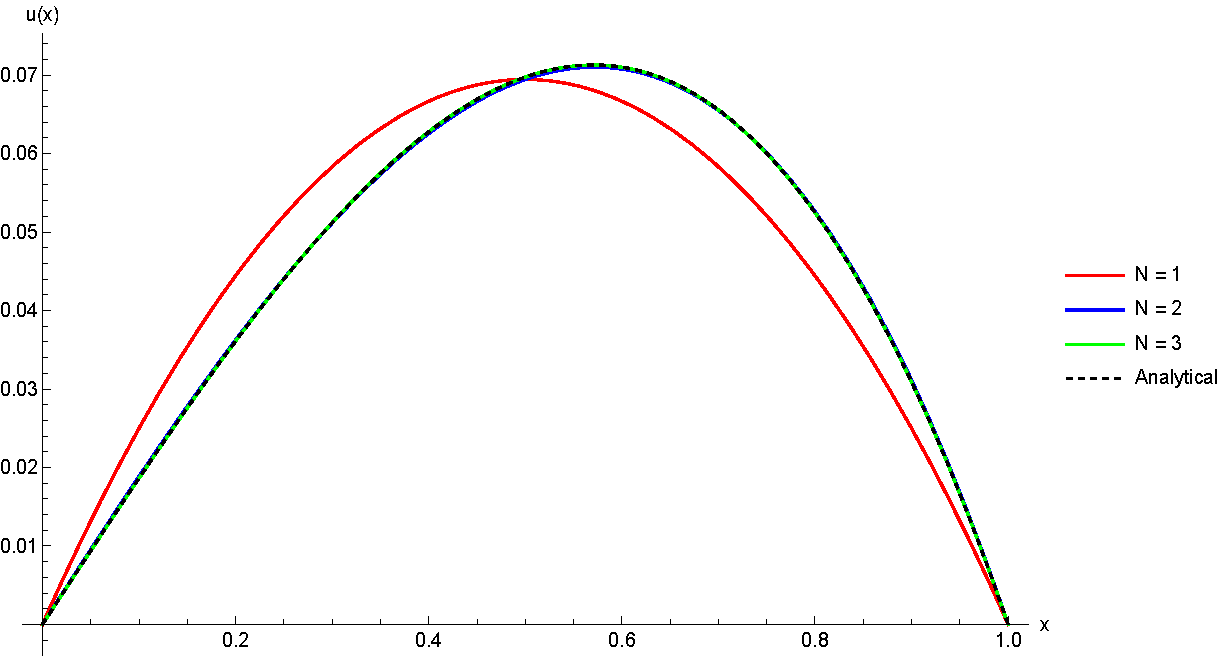
\includegraphics[width=0.7\textwidth]{3.pdf}
        \caption{График полученных решений при различных N}
    \end{figure}
    \begin{figure}[h]
        \centering
        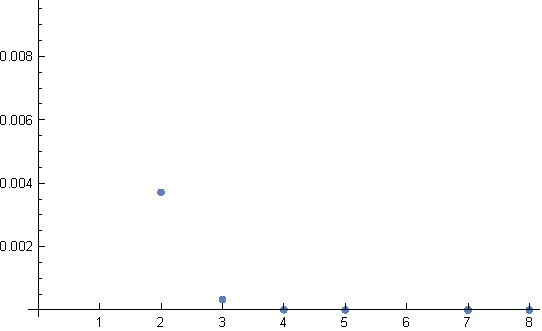
\includegraphics[width=0.5\textwidth]{3_error.pdf}
        \caption{График ошибок}
    \end{figure}

    \pagebreak

    \section{ Метод Галеркина}

    \begin{center}
        \begin{tabular}{|c|c|c|} 
         \hline
         № & Норма ошибки & Коэффициенты \\ 
         \hline
         1 & $0.115$ & $a_1=0.2778$ \\ 
         \hline
         2 & $0.0037$ & $a_1=0.1924, a_2=0.1707$ \\ 
         \hline
         3 & $3\cdot10^{-4}$ & $a_1=0.1878, a_2=0.1941, a_3=-0.02341$ \\ 
         \hline
         4 & $7.2\cdot10^{-6}$ & $a_1=0.1884, a_2=0.1886, a_3=-0.01052, a_4=-0.0086$ \\ 
         \hline
         5 & $4.1\cdot10^{-7}$ & $a_1=0.1884, a_2=0.1884, a_3=-0.0095, a_4=-0.01, a_5=0.0008$ \\ 
         \hline
        \end{tabular}
    \end{center}

    \begin{figure}[h]
        \centering
        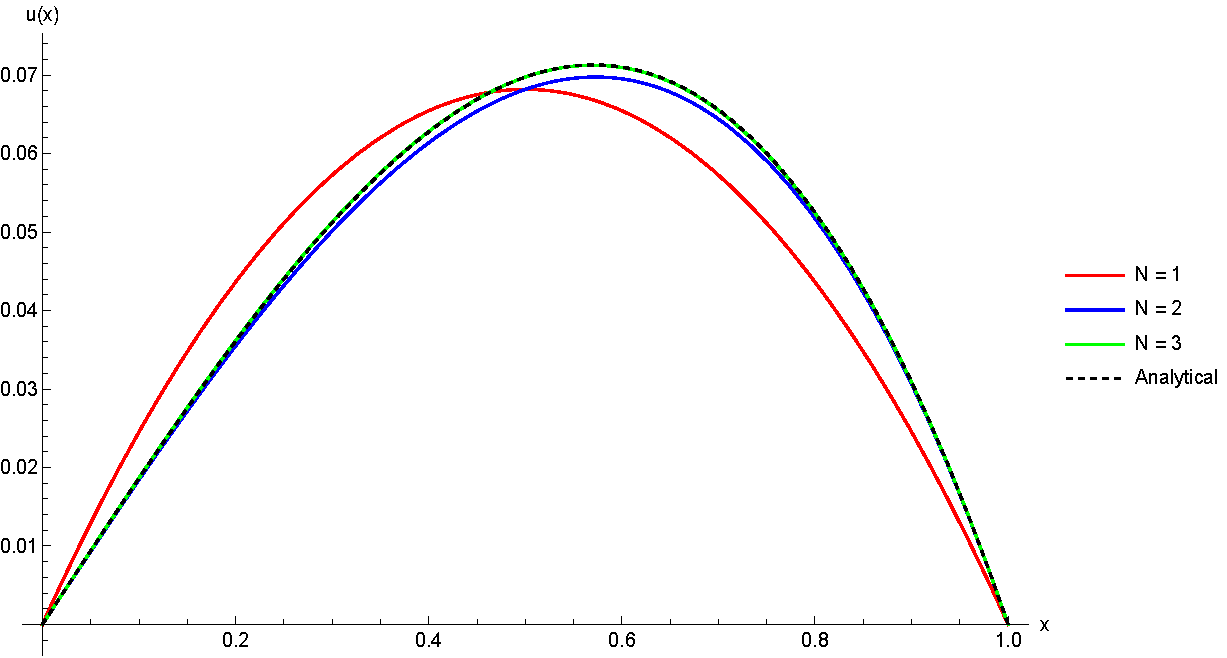
\includegraphics[width=0.7\textwidth]{4.pdf}
        \caption{График полученных решений при различных N}
    \end{figure}
    \begin{figure}[h]
        \centering
        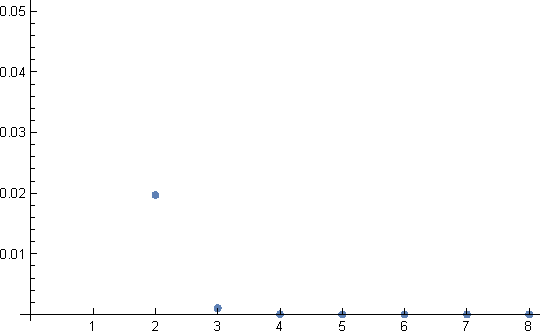
\includegraphics[width=0.5\textwidth]{4_error.pdf}
        \caption{График ошибок}
    \end{figure}

    \pagebreak

    \section{Метод наименьших квадратов}

    \begin{center}
        \begin{tabular}{|c|c|c|} 
         \hline
         № & Норма ошибки & Коэффициенты \\ 
         \hline
         1 & $0.117$ & $a_1=0.2723$ \\ 
         \hline
         2 & $0.021$ & $a_1=0.1875, a_2=0.1695$ \\ 
         \hline
         3 & 1$3\cdot10^{-3}$ & $a_1=0.1884, a_2=0.1928, a_3=-0.02332$ \\ 
         \hline
         4 & $2\cdot10^{-5}$ & $a_1=0.1884, a_2=0.1885, a_3=-0.01046, a_4=-0.008571$ \\ 
         \hline
         5 & $1.23\cdot10^{-6}$ & $a_1=0.1884, a_2=0.1884, a_3=-0.0095, a_4=-0.01, a_5=0.0008$ \\ 
         \hline
        \end{tabular}
    \end{center}

    \begin{figure}[h]
        \centering
        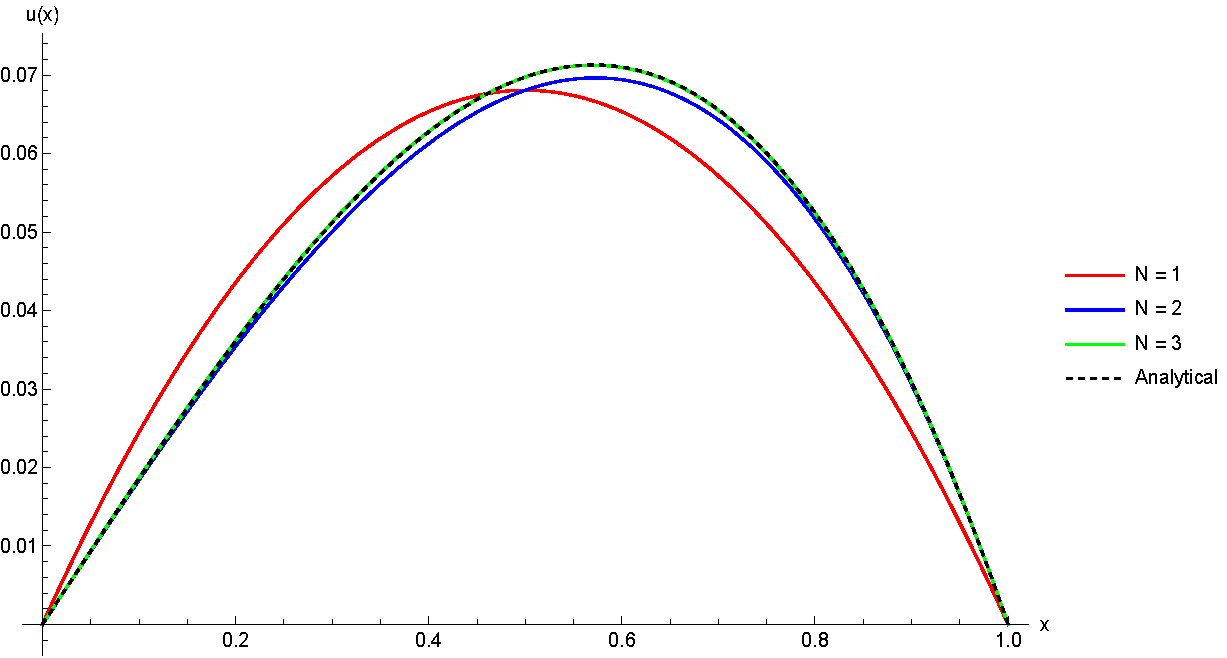
\includegraphics[width=0.7\textwidth]{5.pdf}
        \caption{График полученных решений при различных N}
    \end{figure}
    \begin{figure}[h]
        \centering
        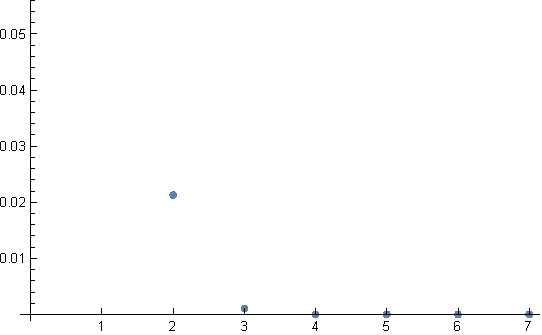
\includegraphics[width=0.5\textwidth]{5_error.pdf}
        \caption{График ошибок}
    \end{figure}

    \pagebreak

    \section{Метод Ритца}

    \begin{center}
        \begin{tabular}{|c|c|c|} 
         \hline
         № & Норма ошибки & Коэффициенты \\ 
         \hline
         1 & $0.115$ & $a_1=0.2778$ \\ 
         \hline
         2 & $0.004$ & $a_1=0.1924, a_2=0.1707$ \\ 
         \hline
         3 & $3\cdot10^{-4}$ & $a_1=0.1878, a_2=0.1941, a_3=-0.02341$ \\ 
         \hline
         4 & $7.2\cdot10^{-6}$ & $a_1=0.1884, a_2=0.1886, a_3=-0.01052, a_4=-0.0086$ \\ 
         \hline
         5 & $4.1\cdot10^{-7}$ & $a_1=0.1884, a_2=0.1884, a_3=-0.0095, a_4=-0.01, a_5=0.0008$ \\ 
         \hline
        \end{tabular}
    \end{center}

    \begin{figure}[h]
        \centering
        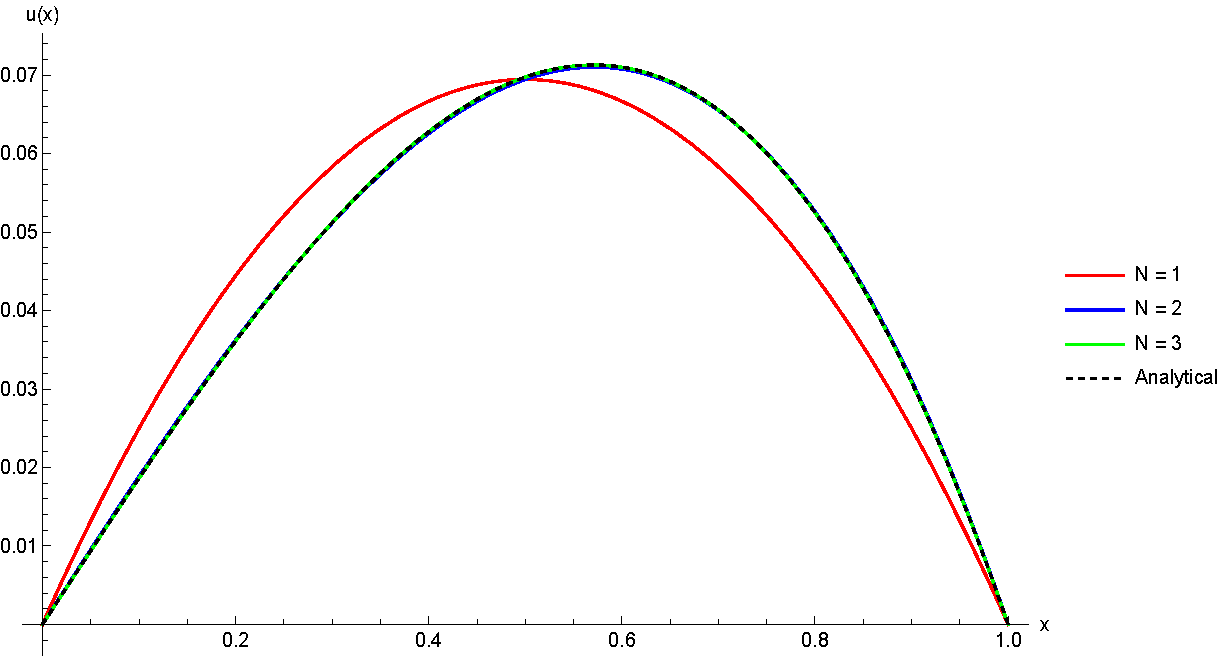
\includegraphics[width=0.7\textwidth]{6.pdf}
        \caption{График полученных решений при различных N}
    \end{figure}
    \begin{figure}[h]
        \centering
        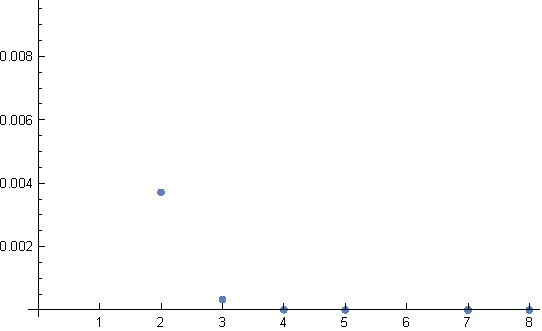
\includegraphics[width=0.5\textwidth]{6_error.pdf}
        \caption{График ошибок}
    \end{figure}

    \section{Выводы}

    Рассмотренные проекционные методы дают достаточно высокую точность. Наилучшую точность дает метод Бубнова-Галеркина. В среднем, для получения относительной ошибки $10^{-4}-10^{-3}$ требуется взять 3 слагаемых в разложении по базисным функциям.

\end{document}

% \begin{center}
%     \begin{tabular}{|c|c|c|} 
%      \hline
%      № & Норма ошибки & Коэффициенты \\ 
%      \hline
%      1 & $0.$ & $a_1=$ \\ 
%      \hline
%      2 & $0.$ & $a_1=, a_2=$ \\ 
%      \hline
%      3 & $\cdot10^{-4}$ & $a_1=, a_2=, a_3=$ \\ 
%      \hline
%      4 & $\cdot10^{-5}$ & $a_1=, a_2=, a_3=, a_4=$ \\ 
%      \hline
%      5 & $\cdot10^{-6}$ & $a_1=, a_2=, a_3=, a_4=, a_5=$ \\ 
%      \hline
%     \end{tabular}
% \end{center}